
\section{Manifestation of Modbus protocol through \scilab}
The objective of this experiment is to make the user acquainted with
the demonstration of Modbus protocol through the Scilab-Arduino toolbox. 
It gives an insight into how to acquire readings from the energy meter and interpret them accordingly. As explained in \secref{sec:energy-meter}, 
an energy meter is a device that gives us different electrical parameters, including voltage, current, and power, consumed by a device. Here, we aim to obtain these values using the Scilab-Arduino toolbox. For data transmission, we have used an RS485 module.

Scilab is used for giving the required parameters to \arduino. For
example, the user will tell the required slave address to be accessed
and the number of registers to be read from or written to. Here,
\arduino\ acts as a master and energy meter as a slave. Therefore,
referring to a particular slave address will refer to the registers
that hold the desired electrical parameters (current, voltage, power, etc.), which we want to read from the energy meter.

In this experiment, \arduino\ is connected to the energy meter via an RS485 module which facilitates long-distance communication. 
\scilab\ sends the RQ to the \arduino\, which in turn sends it to the
energy meter. The energy meter then accesses the values in the
required addresses in its memory and transfers them back. This again
is in the form of another packet called RP. In this packet, the data is stored in a little-endian hexadecimal format. Thus, we make use of IEEE 754 to obtain the decimal value from this data. 


% \subsection{Software for the experiment}
% Apart from the Scilab-Arduino toolbox, the software for this experiment comprises two parts:
% \begin{enumerate}
% \item  Firmware for \arduino: This firmware is needed to communicate
% with Scilab (using serial interface), and with RS485 module (using
% Software Serial interface). Control logic to enable receive and
% transmit modes of MAX485 chip is also present in this firmware. \figref{fig:modbus-firmware} demonstrates the overall implementation of this firmware.

% \begin{figure}
%   \centering
%   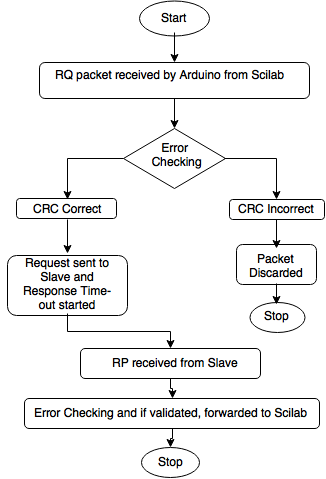
\includegraphics[width=\lgfig]{\LocMODfig/arduino_code_flowchart.png}
%   \caption{Flowchart of Arduino firmware}
%   \label{fig:modbus-firmware}
% \end{figure}

% \item Scilab code: This code requests the parameters in the energy meter
% by sending an RQ to \arduino\ from Scilab. Then it waits till
% an RP is available from the \arduino. After receiving the RP, it extracts 
% the data from this packet and converts it into IEEE
% 754 floating-point format. The overall implementation is being
% described below:
% \begin {enumerate}
% \item Frame an RQ to be sent to the energy meter (slave) in ASCII coded decimal
% format. 
% \item Send the RQ serially to \arduino. 
% \item Let \arduino\ send the RQ to the energy meter via RS485 module. 
% \item Let the energy meter send the RP to \arduino\ via RS485 module. 
% \item Read the RP available on \arduino. 
% \item Extract the data stored in holding registers from the RP. 
% \item Assuming this data to be stored in little-endian format, 
% convert this data in floating-point values using IEEE 754 standard. 
% \item Display the value in the \scilab\ Console. 
% \end{enumerate}
% \figref{fig:flow-chart} presents the sequence in which the steps mentioned above are executed. 
% \begin{figure}
%   \centering
%   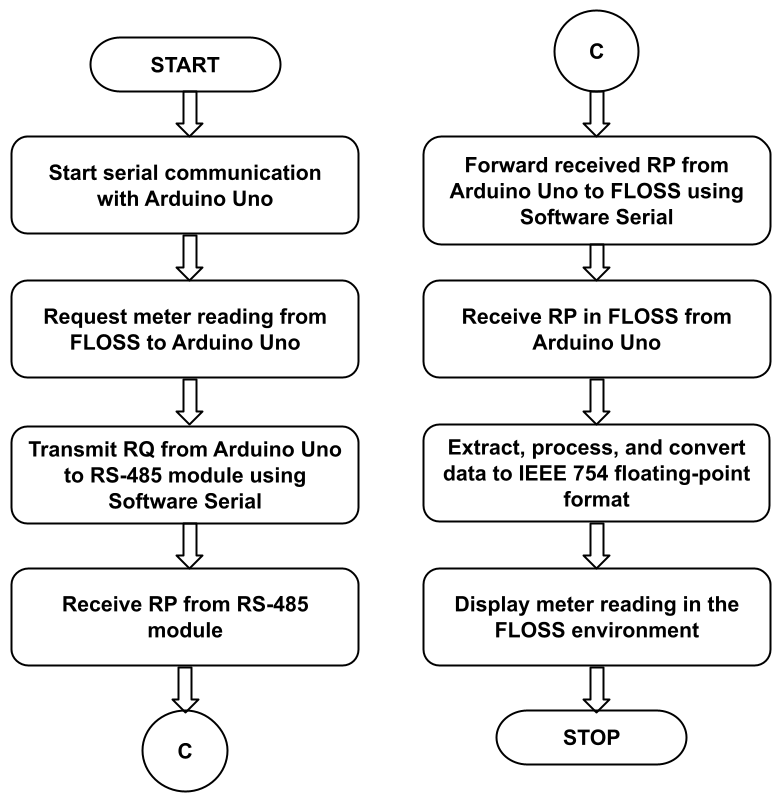
\includegraphics[width=\hgfig]{\LocMODfig/flowchart.png}
%   \caption{Flowchart of the steps happening in Scilab code}
%   \label{fig:flow-chart}
% \end{figure}

% \end{enumerate}

% In output, user could see the requested energy parameter on Scilab
% console. For demonstration we have taken single phase current, single
% phase voltage and single phase active power reading. We can always
% verify the Scilab output with the value being displayed on the Energy
% Meter display screen.


\section{Reading the electrical parameters from Scilab}
\subsection{Reading the electrical parameters}
In this section, we will show how to access the three parameters (voltage, current, and active power) in the energy meter. As discussed above, we will send an RQ from Scilab to \arduino. Subsequently, \arduino\ will provide us with an RP, which can be decoded to extract the desired parameter. The reader should go through the instructions given in \secref{sec:sci-start} before getting started. 

% \subsection{Arduino Firmware}
% \label{sec:firmware-modbus}
% \addtocontents{ard}{\protect\addvspace{\codclr}}
% \begin{ardcode}
%   \acaption{First 10 lines of the firmware for Modbus Energy Meter
%     experiment}
%   {First 10 lines of the firmware for Modbus.  Available at
%     \LocMODardbrief{send\_packet.ino}.}
%   \label{ard:firmware-modbus}
%   \lstinputlisting[firstline=1,lastline=10]
%   {\LocMODardcode/send_packet.ino}
% \end{ardcode}

\subsection{Scilab Code}
\label{sec:modbus-scilab-code}
\addtocontents{cod}{\protect\addvspace{\codclr}}

\begin{scicode}
  \ccaption{First 10 lines of the function for scifunc block}
  {First 10 lines of the Scifunc block function.  Available at
    \LocMODscibrief{read\_val.sci}.}
  \label{sci:val-modbus}
  \lstinputlisting[firstline=1,lastline=10]
  {\LocMODscicode/read_val.sce}
\end{scicode}

\begin{scicode}
  \ccaption{First 10 lines of the code for Single Phase Current Output}
  {First 10 lines of the code for Single Phase Current Output.
    Available at \LocMODscibrief{read\_current.sci}.}
  \label{sci:current-modbus}
  \lstinputlisting[firstline=1,lastline=10]
  {\LocMODscicode/read_current.sci}
\end{scicode}

\begin{scicode}
  \ccaption{First 10 lines of the code for Single Phase Voltage Output}
  {First 10 lines of the code for Single Phase Voltage Output.
    Available at \LocMODscibrief{read\_voltage.sci}.}
  \label{sci:voltage-modbus}
  \lstinputlisting[firstline=1,lastline=10]
  {\LocMODscicode/read_voltage.sci}
\end{scicode}

\begin{scicode}
  \ccaption{First 10 lines of the code for Single Phase Active Power
    Output}{First 10 lines of the code for Single Phase Active Power
    Output.  Available at
    \LocMODscibrief{read\_active\_power.sci}.}
  \label{sci:modbus-power}
  \lstinputlisting[firstline=1,lastline=10]
  {\LocMODscicode/read_active_power.sci}
\end{scicode}

\paragraph{Note: } After we send the RQ from Scilab to the energy meter, we will receive an RP from the energy meter. RP contains the data requested. This data
is read serially in Scilab and the bytes so received are stored in a variable. On analyzing the bytes received, we observe some blank spaces received along with the data. So the required data starts from the fourth byte available, excluding spaces. For example, If there are {\tt n} spaces received before the packet, so the required data would be available from {\tt (n+4)}th position onwards. It means that we have to analyze the four bytes starting at {\tt (n+4)}th position. Note that the RP may have one or more spaces at the start or the end. That's why we may have to shift our index to extract the desired data. 

\subsection{Output in the Scilab Console}
In this section, we present the results. In this experiment, the three parameters: voltage, current, and active power in the energy meter have been accessed and displayed on the Scilab console. For each of these three parameters, we present two image: one showing the reading being shown in the energy meter and the another showing the value being displayed in the Scilab Console. 
\begin{enumerate}
  \item Single phase current output: \figref{fig:current-console} and
        \figref{fig:current-meter} show Scilab code output of current in
        Amperes and corresponding snapshot of energy meter display with a
        single load rated 60W-230V.
        
        \begin{figure}
          \centering
          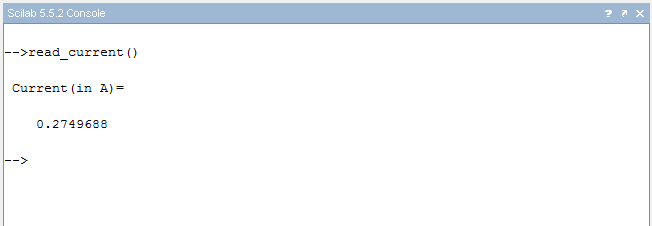
\includegraphics[width=\linewidth]{\LocMODfig/current-output.png}
          \caption{Single phase current output on Scilab Console}
          \label{fig:current-console}
        \end{figure}
        
        \begin{figure}
          \centering
          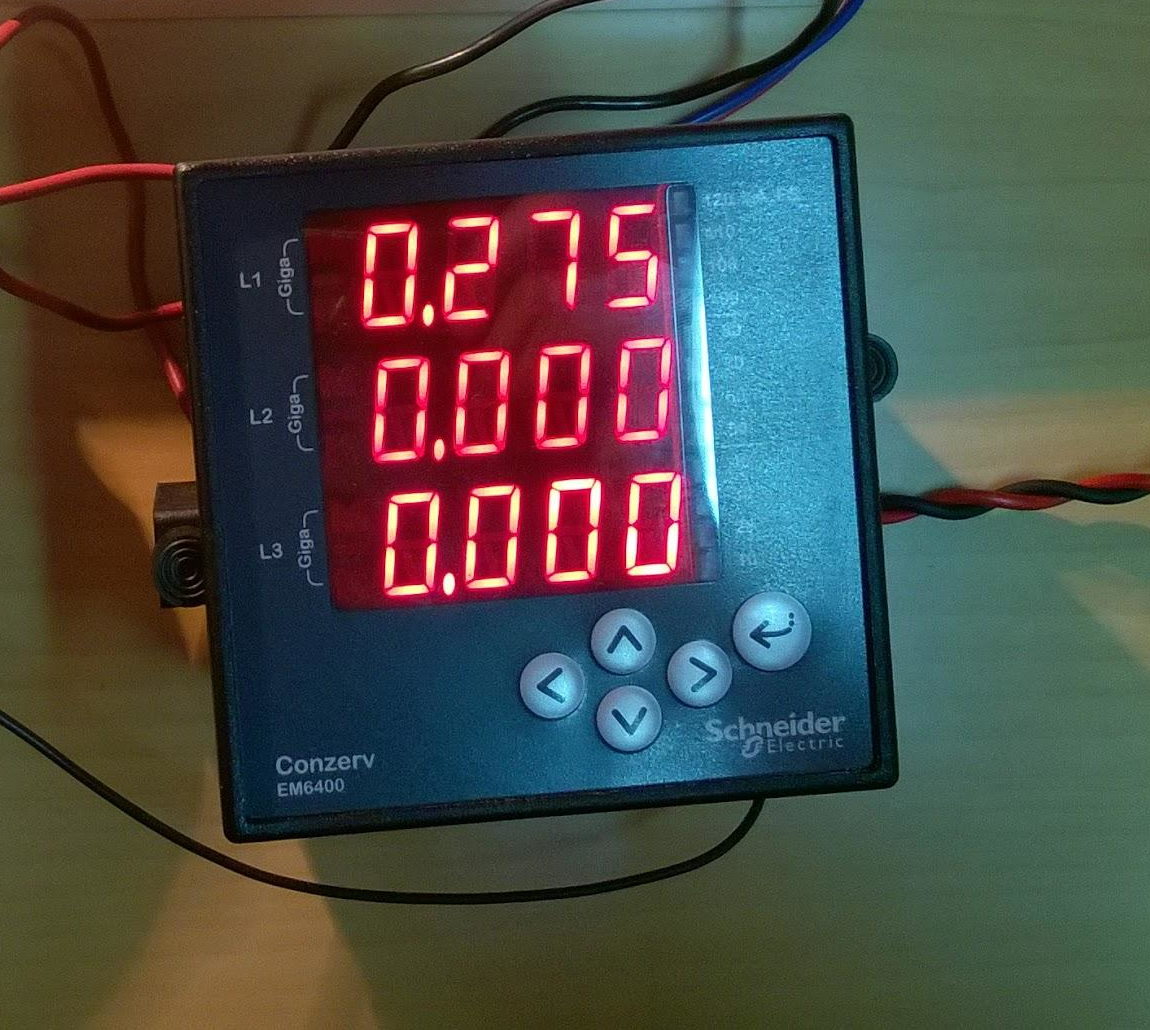
\includegraphics[width=\lgfig]{\LocMODfig/current-output-setup.jpg}
          \caption{Single phase current output in energy meter}
          \label{fig:current-meter}
        \end{figure}
        
  \item Single phase voltage output: \figref{fig:voltage-console} and
        \figref{fig:voltage-meter} show Scilab code output of voltage in
        Volts and corresponding snapshot of energy meter display with a
        single load rated 60W-230V.
        
        \begin{figure}
          \centering
          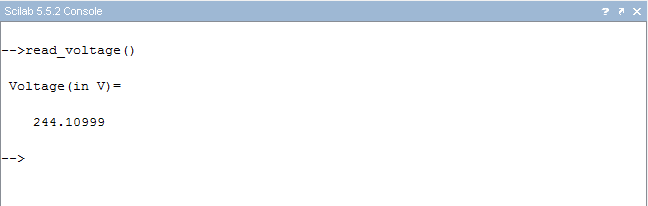
\includegraphics[width=\linewidth]{\LocMODfig/voltage-output.png}
          \caption{Single phase voltage output on Scilab Console}
          \label{fig:voltage-console}
        \end{figure}
        
        \begin{figure}
          \centering
          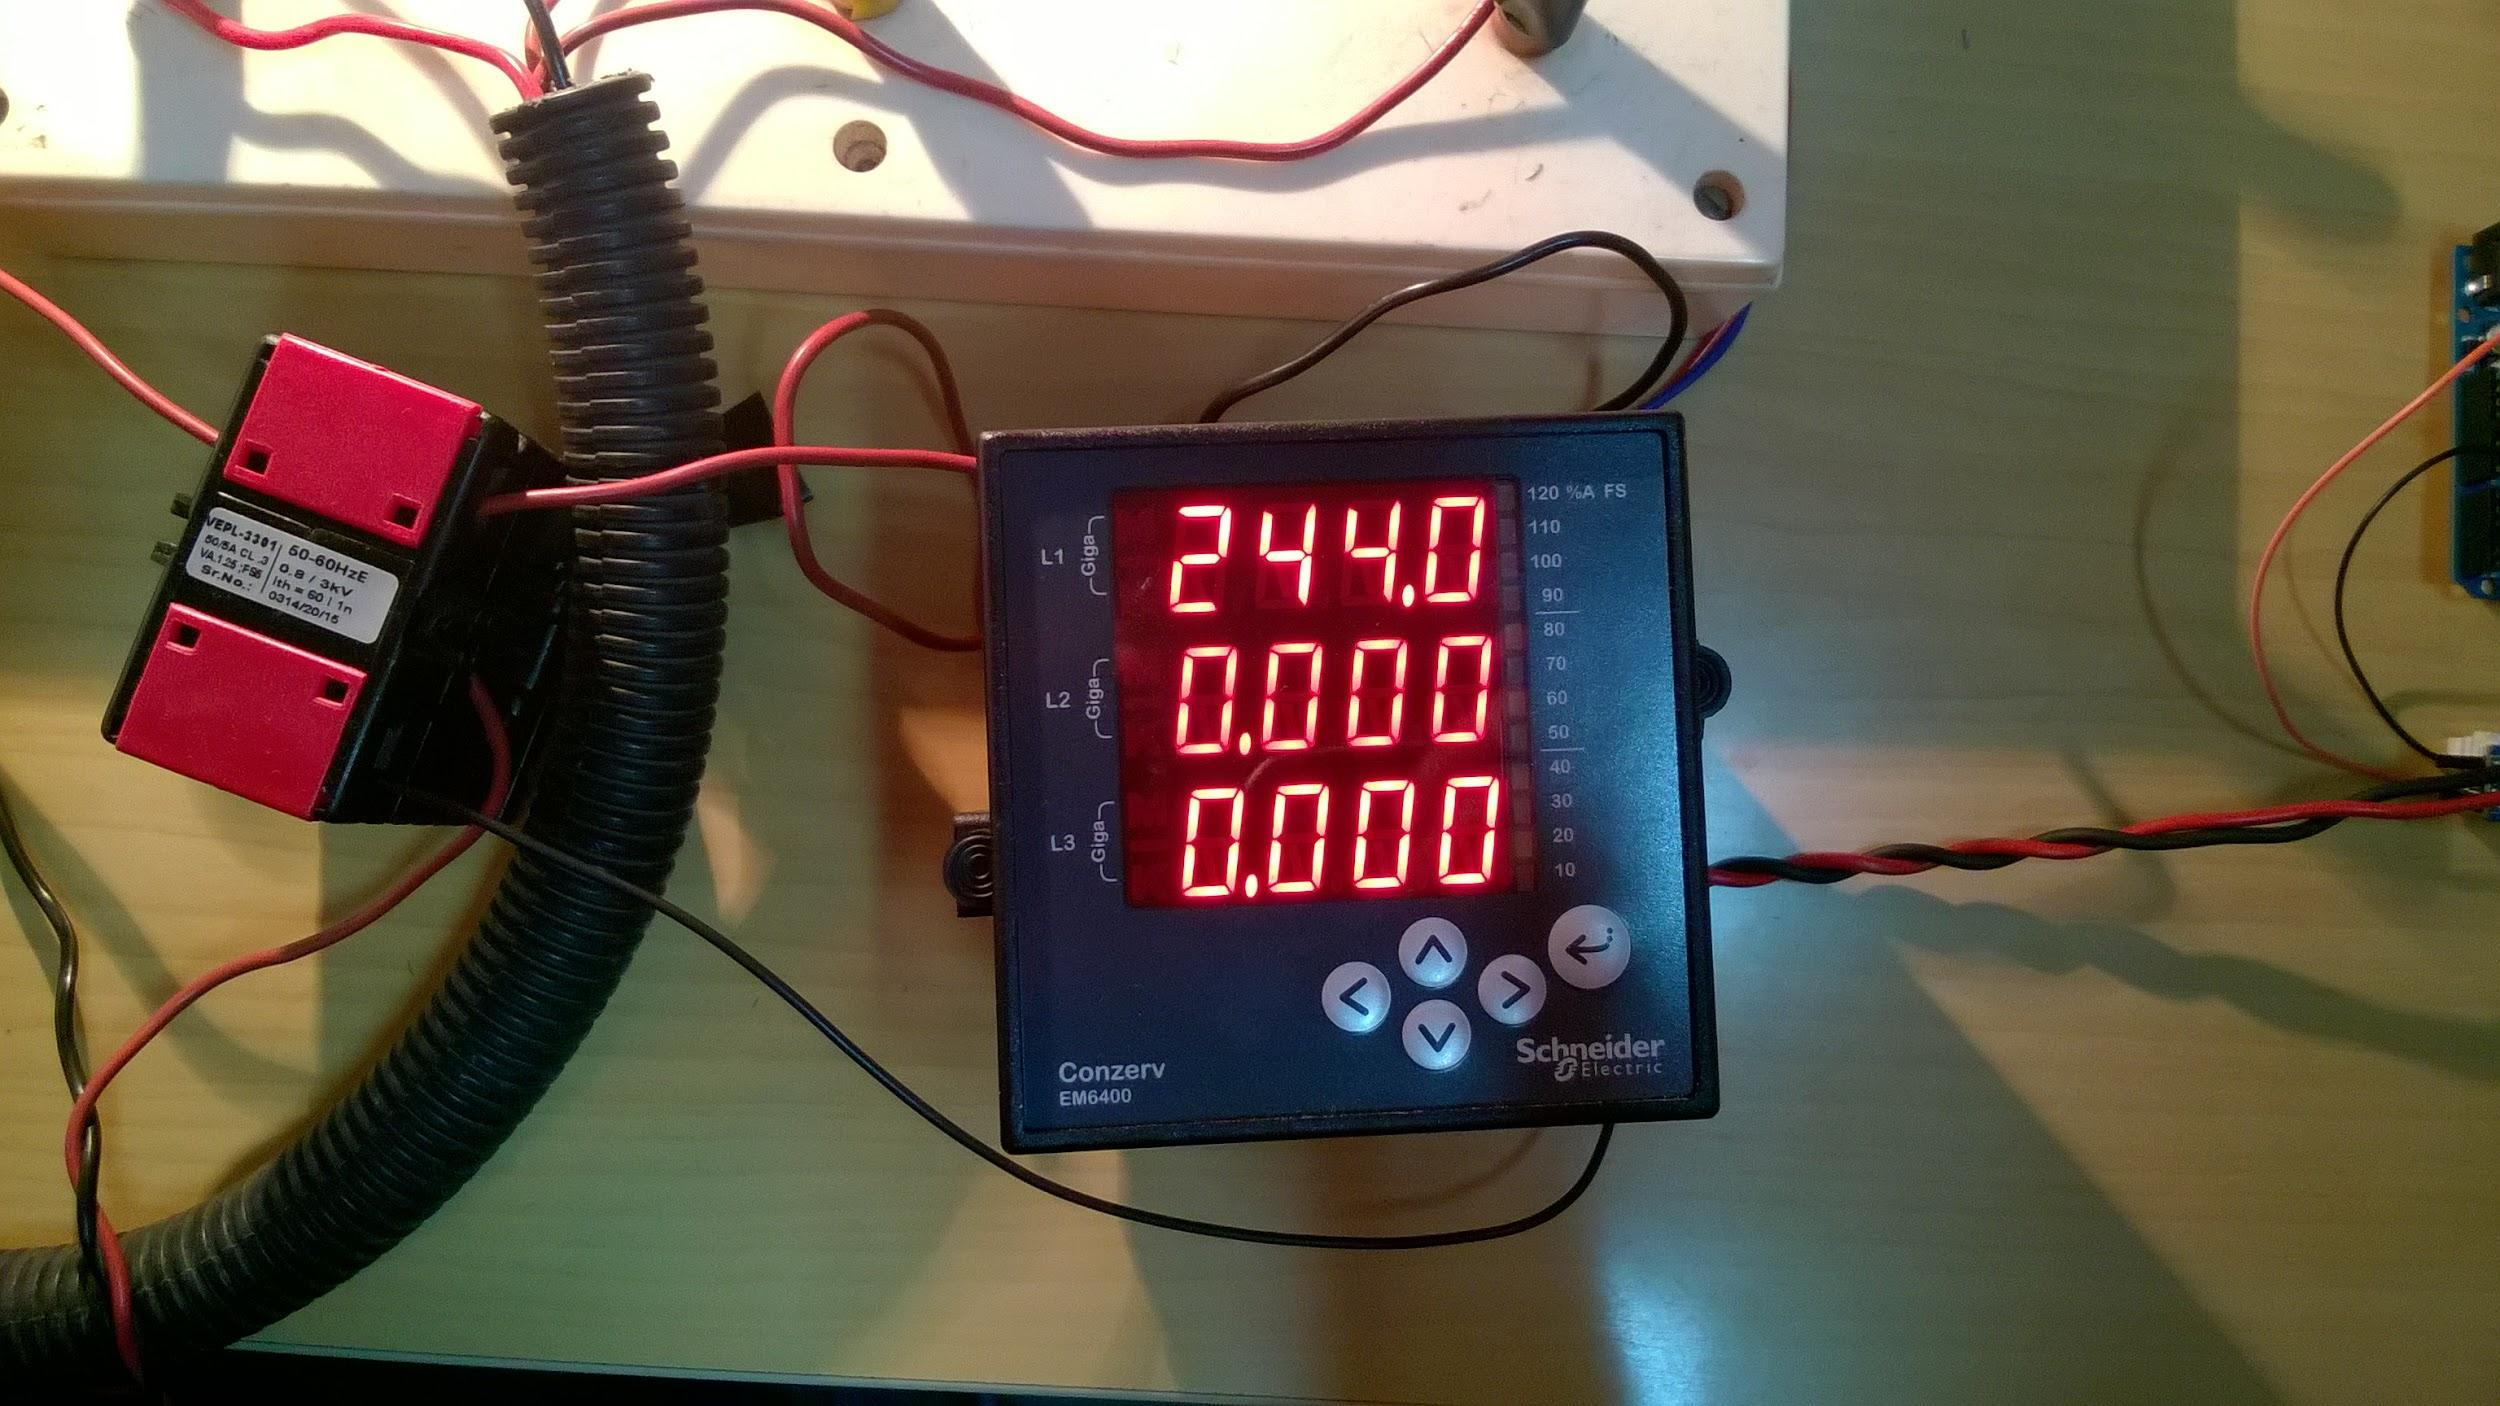
\includegraphics[width=\lgfig]{\LocMODfig/voltage-output-setup.jpg}
          \caption{Single phase voltage output in energy meter}
          \label{fig:voltage-meter}
        \end{figure}
        
  \item Single phase active power output:  \figref{fig:power-console} and \figref{fig:power-meter} show Scilab code output of active power
        in Watts and corresponding snapshot of energy meter display with a
        single load rated 60W-230V.        
        \begin{figure}
          \centering
          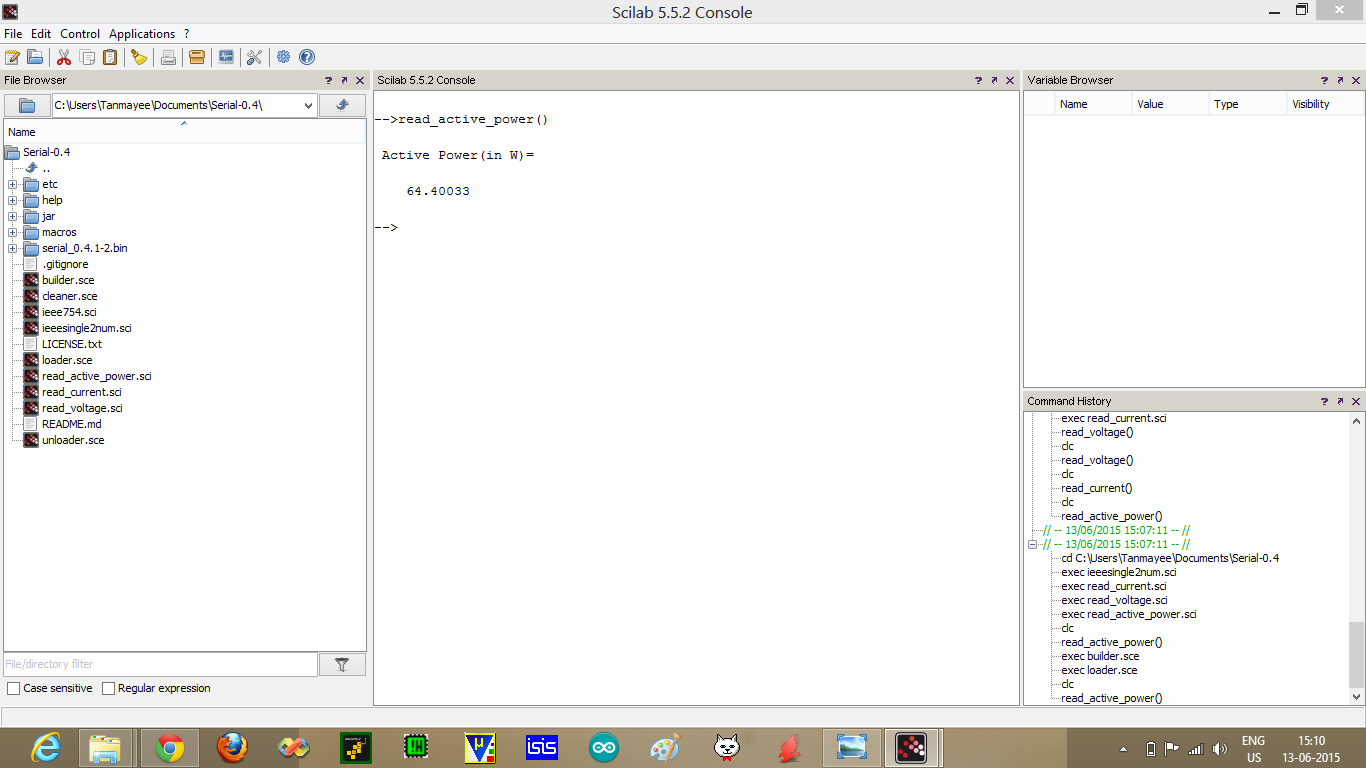
\includegraphics[width=\linewidth]{\LocMODfig/active-power-output.png}
          \caption{Single phase active power output on Scilab Console}
          \label{fig:power-console}
        \end{figure}
        
        \begin{figure}
          \centering
          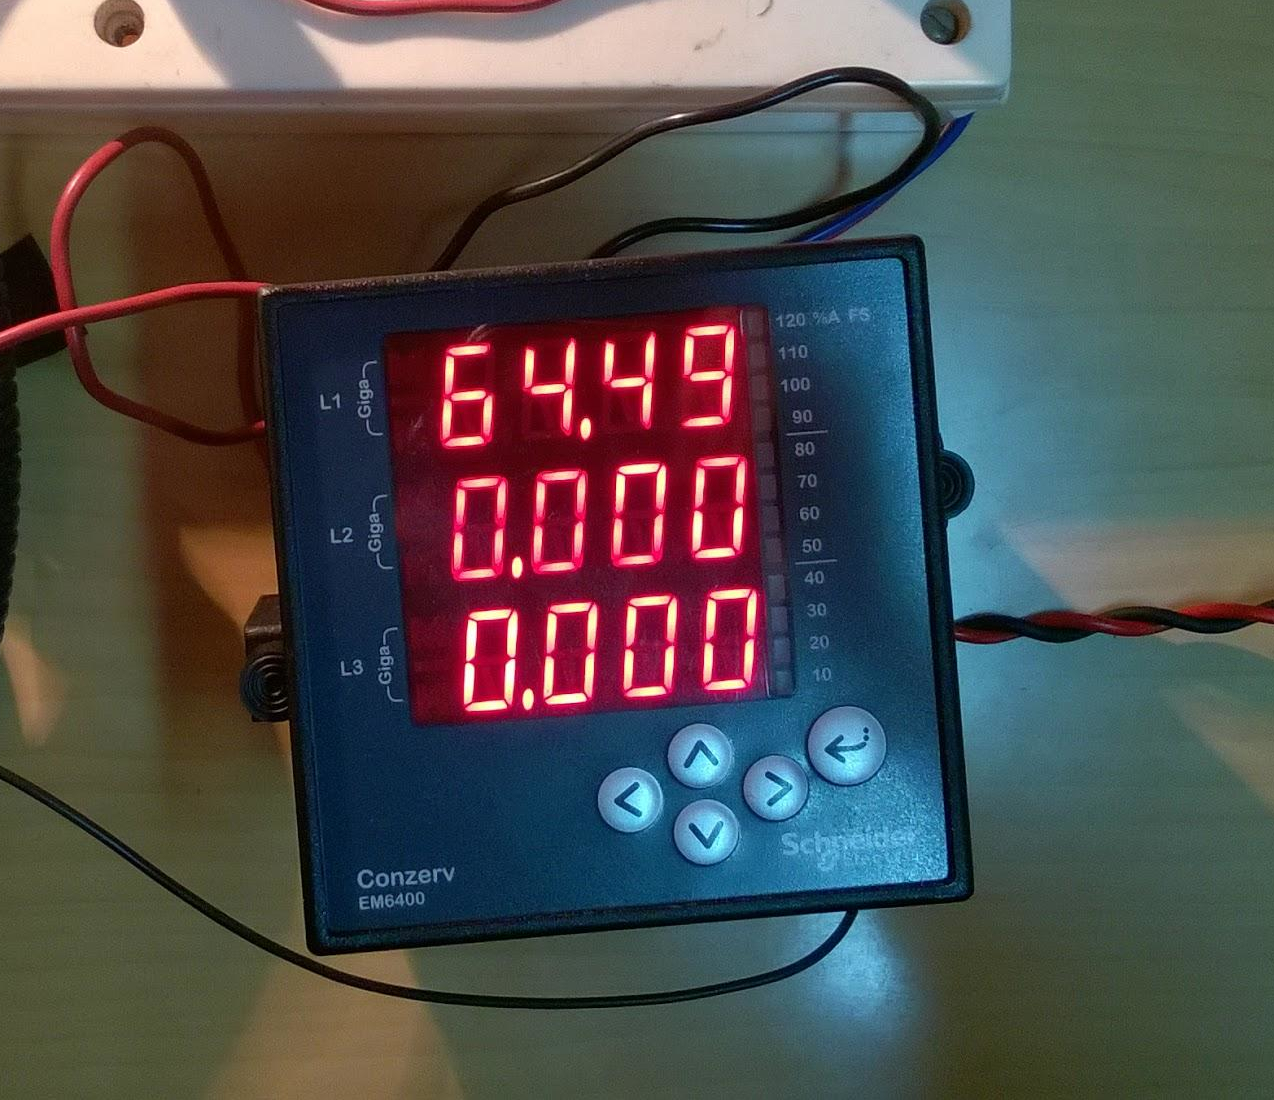
\includegraphics[width=\lgfig]{\LocMODfig/active-power-output-setup.jpg}
          \caption{Single phase active power output in energy meter}
          \label{fig:power-meter}
        \end{figure}
        
\end{enumerate}


\section{Reading the electrical parameters from Xcos}
In this section we will carry out the same experiments discussed in
the previous sections but through Xcos. One should go through
\secref{sec:xcos-start} before continuing.

\begin{enumerate}
  \item The Xcos diagram for performing the read values for single phase
        current, single phase voltage and single phase power operation is as
        shown in \figref{fig:mod-read}. The location of the xcos file is
        mentioned in the caption of the figure.
        
        \begin{figure}
          \centering
          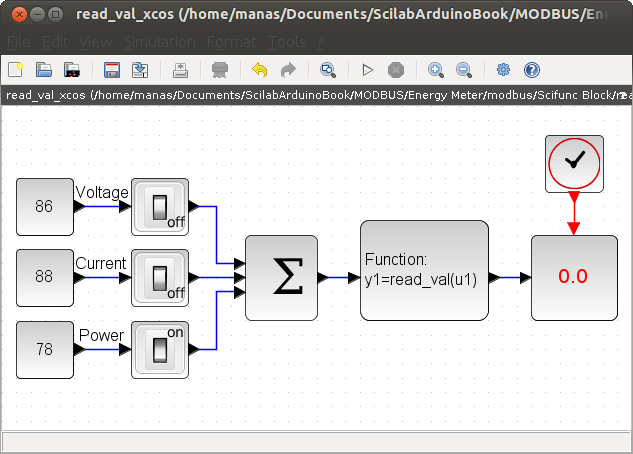
\includegraphics[width=\lgfig]{\LocMODfig/read_value_xcos.png}
          \caption[Xcos diagram to read Energy Meter values]{Xcos diagram to
            read Energy Meter values.  This is what one sees when {\tt
                \LocMODscibrief/read\_value\_xcos.zcos} is invoked.}
          \label{fig:mod-read}
        \end{figure}
        The parameters of the blocks can be changed by right clicking on the
        block and choosing {\tt Block Parameters}. One can also double click
        on the block. The values for each block is tabulated in
        \tabref{tab:mod-xcos-read}.  All other parameters are to be left
        unchanged.
        
        \begin{table}
          \centering
          \caption{Xcos parameters to read Energy Meter}
          \label{tab:mod-xcos-read}
          \begin{tabular}{llc} \hline
            Name of the block & Parameter name                               & Value           \\ \hline
            CONST\_m          & Address byte for voltage                     & 86              \\
                              & Address byte for current                     & 88              \\ 
                              & Address byte for power                       & 78              \\ \hline
            SELF\_SWITCH      & Signal Routing                               & on/off          \\ \hline
            BIGSOM\_f         & Scalar vector addition/subtraction Summation & [1;1;1]         \\ \hline
            scifunc\_block\_m & Block for user\-defined function             & read\_value.sci \\ \hline 
            AFFICH\_m         & Block inherits(1) or not (0)                 & 0               \\ \hline
            CLOCK\_c          & Period                                       & 0.1             \\
                              & Initialisation Time                          & 0               \\ \hline
          \end{tabular}
        \end{table}
\end{enumerate}


